\documentclass[journal,twoside,web]{ieeecolor}
\usepackage{generic}
\usepackage{cite}
\usepackage{amsmath,amssymb,amsfonts}
\usepackage{algorithmic}
\usepackage{graphicx}
\usepackage{textcomp}
\usepackage{url}


\usepackage{float}
\usepackage{xcolor}
\usepackage{booktabs}
\usepackage{tabularx}
\usepackage{siunitx}
\usepackage{listings}


\definecolor{codegreen}{rgb}{0,0.6,0}
\definecolor{codegray}{rgb}{0.5,0.5,0.5}
\definecolor{codepurple}{rgb}{0.58,0,0.82}
\definecolor{backcolour}{rgb}{0.95,0.95,0.92}
\lstdefinestyle{mystyle}{
    backgroundcolor=\color{backcolour},   
    commentstyle=\color{codegreen},
    keywordstyle=\color{magenta},
    numberstyle=\tiny\color{codegray},
    stringstyle=\color{codepurple},
    literate=
    {\{}{{{\color{red}\{}}}1
    {\}}{{{\color{red}\}}}}1
    {[}{{{\color{red}[}}}1
    {]}{{{\color{red}]}}}1
    {)}{{{\color{red})}}}1
    {(}{{{\color{red}(}}}1,
    basicstyle=\ttfamily\footnotesize,
    breakatwhitespace=false,         
    %breaklines=true,                 
    captionpos=b,                    
    keepspaces=true,                 
    numbers=left,                    
    numbersep=5pt,                  
    showspaces=false,                
    showstringspaces=false,
    showtabs=false,                  
    tabsize=2
}

\lstset{style=mystyle}


\def\BibTeX{{\rm B\kern-.05em{\sc i\kern-.025em b}\kern-.08em T\kern-.1667em\lower.7ex\hbox{E}\kern-.125emX}}

\begin{document}
%PROPUESTAS DE TÍTULO JESÚS: 
%
%Real-Time, regulation“Real-Time Regulatory-Compliant Drone Navigation for Power Infrastructure Inspection compliance UAS Navigation \\\\
%Bringing Compliance to Flight: A Real-Time Navigation Algorithm for Drone-Based Power Line Inspection\\\\
%A Regulation-Aware Real-Time Navigation Algorithm for UAV-Based Electrical Infrastructure Inspection\\\\
%Design and Validation of a Real-Time, Regulation-Compliant Navigation Algorithm for UAV Inspection of Electrical Infrastructure

\title{Regulatory Compliant Moving Obstacle Avoidance Navigation Algorithm for Drone-Based Power Line Inspection}
\author{Pablo De Porcellinis \thanks{Pablo de Porcellinis is with FuVeX Civil SL and the Mathematical Engineering and Computer Science Department at the Public University of Navarre, Spain. (e-mail: p.porcellinis@fuvex.com)}, Xabier Olaz \thanks{Xabier Olaz is with the Mathematical Engineering and Computer Science Department at the Public University of Navarre, Spain.}, and Jes\'us Villadangos \thanks{Jes\'us Villadangos is with the Mathematical Engineering and Computer Science Department at the Public University of Navarre and the Institute of Smart Cities, Public University of Navarre, Spain.}}

\markboth{\journalname, VOL. XX, NO. XX, XXXX}
{Author \MakeLowercase{\textit{et al.}}: Title}


\maketitle



\begin{abstract}
Autonomous UAV obstacle avoidance is not new, but most existing algorithms focus on collision-free flight, geometric efficiency, or dynamic feasibility. Much less work addresses the European regulatory logic that an autonomous route should avoid exposing uninvolved people and other protected ground parties to unnecessary overflight risk. This paper presents Path Planning and Moving Obstacle Avoidance Regulatory Compliant Evasion, a deterministic real-time local replanning method for waypoint-preserving obstacle avoidance in autonomous power-line inspection missions. The method is implemented and evaluated inside a simulated real environment in Unreal, where it operates together with a waypoint-driven flight controller, a YOLO-based perception front-end, and a  monocular obstacle geopositioning. In the current implementation, civilian-like detections and nearby entities are converted into protected local no-fly regions that trigger conservative detours instead of nominal overflight. Based on the literature reviewed for 2024--2026, we are not aware of a published method that combines this EASA-motivated no-overflight objective with deterministic online local replanning and autonomous power-line inspection integration in the same way. The presented results show the proposed solution as a reproducible, low-overhead, and auditable local replanning method that operationalizes part of the European ground-risk logic at the online controller level, while the simulated workflow provides the integration and validation environment used to characterize its behavior.
\end{abstract}

\begin{IEEEkeywords}
 Ground risk, moving obstacle avoidance, local replanning,Regulation Compliance,  safety-critical navigation, SORA, UAV inspection, uninvolved people.
\end{IEEEkeywords}

\section{Introduction}
\label{sec:introduction}

Unmanned Aerial Vehicles (UAVs) are becoming a practical tool for infrastructure inspection, surveillance, and monitoring, with a growing impact across agriculture, critical infrastructure, and other industrial environments \cite{imran2025environmental,marut2024surveillance}. Power-line inspection is one of the most relevant use cases because it combines long-range navigation, repeated geometric structures, tight mission corridors, and the need to react to unexpected obstacles without compromising the inspection objective. The operational experience of companies such as FuVeX in this scenario helps to identify the remaining gaps. Moreover, it demonstrates the practical value of the solution developed in this research for real-world applications.  %PORCE: comprobar que se ha reflejado la idea que la experiencia de FuVeX ha ayudado a encontrar este gap y que la solución propuesta puede ayudar a solucionar los problemas que a día de hoy se siguen encontrando. 

From a planning point of view, this scenario is difficult because the vehicle must maintain a global mission structure while responding online to local conflicts. Purely global planners are efficient when the environment is static and fully known, but they become brittle under late obstacle appearance or perception uncertainty \cite{debnath2024review,meng2025advances}. On the other hand, fully learned end-to-end policies are harder to audit in safety-critical aeronautical contexts, where traceability and bounded behavior remain important design properties \cite{EASA_AI_Roadmap_2.0}.

The regulatory dimension makes the problem even sharper. Under the UAS regulatory framework of the European Union, the operational core was defined by the Commission Implementing Regulation (EU) 2019/947 on the rules and procedures for the operation of unmanned aircraft and the Commission Delegated Regulation (EU) 2019/945 on unmanned aircraft systems, while, more recently, EASA AMC/GM material now incorporates the JARUS SORA 2.5 package for the `specific' category \cite{EU2019_947,EU2019_945,JARUS_SORA_2_5_2024,EASA_AMC_GM_SORA25_2025}. Within this framework, the acceptability of a route is not only a matter of geometric collision avoidance but also of limiting exposure of uninvolved people and sensitive ground areas. This means that an autonomous planner should not simply ask whether the UAV \emph{can} fly over a location, but whether it \emph{should} do so in a risk-aware operational sense. The existing literature has already started to encode this concern through urban risk maps, third-party risk models, SORA-aware cost functions, and target-level-of-safety constraints \cite{primatesta2019riskaware,primatesta2020groundrisk,pang2022integrated,tang2023thirdparty,zhang2023groundrisk,heinze2023sora,brassel2025riskaware}. However, most of these works remain strategic route optimizers or city-scale risk planners rather than controller-level local replanners for infrastructure inspection missions already in progress.

 The present paper does not claim to encode the full legal tables of open-category separation or the full SORA mitigation calculus within the planner. Instead, it implements the narrower controller-level step that those regulatory mechanisms motivate: live civilian-like detections are converted into temporary protected regions that the UAV should avoid crossing.

 %PORCE: a meter en otra sección como estaba previamente en el otro artículo: Two regulatory details are especially relevant for interpreting the contribution correctly. First, even outside the `specific' category, the European notion of an uninvolved person makes separation a dynamic operational constraint rather than a purely geometric one: as altitude, corridor geometry, and local context change, the practical exclusion region around people on the ground also changes. Second, under SORA 2.5 in the `specific' category, mitigations such as ground observation explicitly reward the capability to detect uninvolved people and avoid overflight in operation \cite{JARUS_SORA_2_5_2024,EASA_AMC_GM_SORA25_2025}.

This paper focuses on Path Planning and Moving Obstacle Avoidance Regulatory Compliant Evasion (PORCE) as the main scientific contribution. The method is a local conflict-resolution system designed for the validated \texttt{SIMULATION} workflow available in the Deep-AeroTwin repository \cite{Deep_Aero_Twin}, where a mission file, a flight controller, an onboard-like perception stack, and a local planner operate together in closed loop. Its role is simple but operationally important: whenever an obstacle enters a conservative reaction horizon, the method temporarily inhibits nominal navigation, computes a bounded local path toward the current mission waypoint, and returns control to the original route as soon as the local conflict disappears. The novelty is therefore not obstacle avoidance in isolation. The novelty is to operationalize a regulatory-aware no-overflight logic for uninvolved third parties and nearby protected entities inside a deterministic, online local replanner. The claim of the paper is correspondingly narrow: the method is advanced as a state-of-the-art contribution in this specific EASA-relevant niche, not as a claim to supersede the broader literature on generic UAV avoidance or strategic risk-aware routing.

The main contributions of the paper are the following.
\begin{itemize}
    \item The definition of PORCE as a deterministic, waypoint-preserving local replanning method for real-time UAV obstacle avoidance in power-line inspection missions, explicitly motivated by European ground-risk and no-overflight concerns.
    \item A formal and reproducible description of how the method is integrated with perception, mission execution, and evaluation of results inside a validated simulation environment.
    
    %PORCE: Creo que este último item sobra en la evalución del artículo ya que el énfasis no está en el hecho de hacer un análisis de la eficacia del código ni auditarlo, sino en buscar una solución realista. 
    %\item An evidence-driven evaluation of the method grounded on repository artifacts, including controlled ablation logs and an audited case study with figures, tables, and derived metrics.

\end{itemize}


\section{State of the Art, Regulatory Concerns, and Research Gap}

\subsection{State of the Art}

Vision-based UAV navigation has been widely studied as a perception-driven alternative to map-only planning, with applications ranging from localization to obstacle detection and local trajectory generation. Although these techniques are often motivated by scenarios where Global Navigation Satellite Systems (GNSS) signals are unavailable, unreliable, or degraded, the literature has demonstrated that vision-based approaches are not limited to such conditions \cite{arafat2023vision,huang2025investigation}. However, there are general reviews on UAV navigation that integrate this type of techniques and consistently distinguish between global and local path planning paradigms. Global path planning methods assume a sufficiently known environment and compute a static solution in advance based on prior maps or predefined constraints. Classical search algorithms such as Dijkstra or A* have been employed within this paradigm and can perform effectively in fully mapped and static environments \cite{lavalle2006planning}.However, their use as stand-alone solutions without integration with complementary perceptual or reactive components presents significant limitations in real-world missions such as power-line inspection or infrastructure monitoring. In contrast, local path planning approaches generate or adapt trajectories online while the vehicle is moving, allowing immediate reactions to newly perceived environmental elements encountered during flight \cite{debnath2024review,meng2025advances}. More specifically, recent surveys in 2025 and 2026 confirm that the dominant design goals remain collision avoidance, dynamic feasibility, and computational efficiency, while explicit treatment of ground exposure of third-parties is still comparatively rare in runtime planning \cite{merei2025survey,nafees2026review}. The proposed method is explicitly positioned in the online local-replanning class.

However, there is a second distinction that matters for this paper and that was often implicit in earlier project notes: much of the academic literature is still evaluated under what may be called a \emph{toy-problem bias}. In those formulations, the navigation problem is simplified enough to validate a planner mathematically, but the same simplifications weaken direct transfer to operational infrastructure inspection. Three simplifications are especially consequential here.
\begin{itemize}[leftmargin=1.3em]
    \item \textbf{Obstacle homogeneity.} Obstacles are often represented as interchangeable geometric primitives or generic occupied cells. In inspection practice, this is not operationally neutral: a tower, a cow, and an uninvolved person may all occupy space, but they do not carry the same legal or operational meaning.
    \item \textbf{Binary safety.} Many planners implicitly treat a mission as successful as long as physical collision is avoided. For European civil UAS operations, that criterion is too weak because a near overflight of uninvolved people may already be operationally unacceptable even when no impact occurs \cite{EU2019_947,JARUS_SORA_2_5_2024,EASA_AMC_GM_SORA25_2025}.
    \item \textbf{Free-space permissiveness.} Conventional local planning usually assumes that any geometrically free air volume is candidate flight space. In European operations, parts of that free volume may still be undesirable or prohibited once uninvolved people, sensitive ground areas, or risk buffers are considered.
\end{itemize}
This is why the present paper does not frame the problem as generic collision avoidance alone. It frames it as online mission execution under geometric and regulatory pressure at the same time.

For power-line inspection, the local planning problem is more operational than academic. The vehicle must continue progressing through a mission corridor while structures, animals, vehicles, or uninvolved people may appear in the neighborhood of the route. Power-line inspection has therefore developed its own system literature, from UAV-image approaches for corridor measurement and obstacle localization \cite{zhang2017powerline} to line detection in cluttered scenes \cite{zhang2019powerlines}, LiDAR-supported automatic inspection \cite{guan2021uavlidar}, dual-view stereovision for reconstruction and clearance estimation \cite{zhou2022dualview}, and dedicated reviews of UAV-enabled power-line inspection \cite{mendu2025state}. On the perception side, Bellou \emph{et al.} report YOLOv8-based aerial inspection for towers, conductors, and insulators \cite{bellou2024aerial}, while Faisal \emph{et al.} synthesize more than 70 studies and identify persistent gaps in multimodal fusion and deployment realism \cite{faisal2025deep}. On the planning side, Huang \emph{et al.} propose a hybrid RRT*+DWA method for dynamic obstacle avoidance in UAV-based power inspection \cite{huang2025hybrid}. These works are highly relevant, but their central objective is still efficient and safe inspection autonomy, not explicit no-overflight treatment of uninvolved people under European operational logic.

\subsection{Regulatory Concerns: Uninvolved People and Ground Risk}

To better understand the potentiality of the proposed solution, it is necessary to explain UAS framework defined by Regulations (EU) 2019/947 and 2019/945 and operationalized through AMC/GM plus SORA 2.5 \cite{EU2019_947,EU2019_945,JARUS_SORA_2_5_2024,EASA_AMC_GM_SORA25_2025}. The key concept around regulation is operational risk, so there are topics within this framework that transform navigation into an optimization problem with hard restrictions. The concept of an uninvolved person plays an significant role in the segmentation of categories. EASA defines it as a person who does not participate in the UAS operation or who is not aware of the instructions and safety precautions given to the UAS operator. In contrast to a power-line tower or cable, an "uninvolved person" generates a dynamic risk field in the surrounding space that adds new constraints inside the route planning, so that route geometry cannot be judged independently from who may be under the aircraft and under what conditions. 

The concept of uninvolved people remains a central regulatory objective as risk levels increase and the operational category changes. However, it is addressed through the definition and control of a Ground Risk Buffer, understood as a spatial margin surrounding the Operational Volume. The Ground Risk Buffer is therefore managed through a combination of operational constraints, technical mitigation, and procedural measures, forming an integral element of the overall safety margin that must be taken into account from the path planning perspective. Within this Ground Risk Buffer definition, the Kinetic Energy ($v, m$) and height ($h$) of the UAS represent important limitation parameters. The actual path-planning algorithms optimize the velocity to reduce the mission time ($J{tiempo}$). However, as the velocity increases, the UAS expands the Ground Risk Buffer, according to the formulas of SORA Annex F \cite{JARUS_SORA_2_5_2024}. A standard planner from the literature will accelerate the improvement of efficiency \cite{dong2017efficient}, inadvertently violating the legally required safety margin.

This SORA 2.5 methodology presented by JARUS establishes a set of ground risk mitigation factors that can be applied to reduce the ground risk level of the operation before flight. This reduction in ground risk level is crucial, as it will imply a reduction in the intrinsic risk of a person being stuck by an UA and a reduction in the level of risk of the whole operation and will allow the aircraft to fly over the expected area without the need to pass a certification process.
Inside these strategic mitigations, the 'M1 (C) mitigation-Ground observation' is directly related with the concept of 'uninvolved people'. This mitigation implies that the UAS crew or the systems inside the aircraft itself can observe most of the overflown area, allowing the detection of 'uninvolved people' in the operational area and maneuvering the UA so that the 'uninvolved people' are not overflown \cite{EASA_AMC_GM_SORA25_2025}.

 The present method does not implement the full legal machinery of either level of risk. What it does implement is the controller-level behavior that every level of risk mentioned motivates: when live perception suggests that the current local corridor should not be overflown, the UAV performs a temporary local bypass instead of persisting on the nominal line.

 
A separate strand of literature already addresses this regulatory concerns directly. Primatesta \emph{et al.} propose a risk-aware urban path-planning strategy with off-line and on-line phases driven by risk maps \cite{primatesta2019riskaware}, and later formalize the construction of ground-risk maps for urban UAV operations \cite{primatesta2020groundrisk}. Pang \emph{et al.} optimize routes by integrating third-party risks into a metropolitan cost model \cite{pang2022integrated}. Tang \emph{et al.} explicitly model obstacle risk, fatality risk, and property loss risk in a Min-cost A* framework \cite{tang2023thirdparty}. Pilko \emph{et al.} and Zhu \emph{et al.} extend the discussion toward spatiotemporal and grid-based ground-risk mapping \cite{pilko2023spatiotemporal,zhang2023groundrisk}. Heinze and Uijt de Haag, and more recently Bra{\ss}el \emph{et al.}, push this line closer to current European operations by encoding SORA and TLS concepts into route optimization \cite{heinze2023sora,brassel2025riskaware}. Complementarily, Du \emph{et al.} review safety-risk modeling for civil UAS operations and show how strongly current safety research is centered on assessment and authorization-oriented risk modeling \cite{du2024safetyrisk}.


The most recent SOTA from 2024 to 2026 further sharpens the distinction between strategic risk planning and controller-level reaction. ElSayed and Mohamed (2024) integrate digital-twin airspace discretization with trajectory optimization under legal and operational constraints \cite{elsayed2024digitaltwin}. Pang \emph{et al.} (2024) model dynamic ground-risk uncertainty for safe drone delivery through stochastic route optimization \cite{pang2024stochastic}. Zhou \emph{et al.} (2025) propose a risk-based path-planning scheme for complex air--ground environments \cite{zhou2025riskbased}, while Riedel (2025) reviews detect-and-avoid standards and shows how strongly recent compliance discussions are still centered on air-risk, separation, and certification interfaces rather than overflight of uninvolved people on the ground \cite{riedel2025daa}. Checker \emph{et al.} (2025) review mission planning from a regulatory perspective, but at the swarm and mission-allocation level \cite{checker2025regulatory}. In 2026, Zhu \emph{et al.} move toward adaptive urban airspace allocation under uncertainty \cite{zhu2026adaptive}, and Nafees \emph{et al.} summarize the broader planning landscape while still highlighting real-time adaptation and constraint integration as open challenges \cite{nafees2026review}. Collectively, these works show that the field is advancing quickly, but the newest contributions still concentrate on strategic routing, digital twins, logistics airspace, or standards alignment more than on deterministic local replanning for inspection missions already underway.

\subsection{Research Gap}

\begin{table*}[t]
    \centering
    \footnotesize
    \begin{tabular}{@{}p{0.25\textwidth} p{0.32\textwidth} p{0.32\textwidth}@{}}
        \toprule
        \textbf{Representative work} & \textbf{What it already solves} & \textbf{Remaining gap relative to the proposed method} \\
        \midrule
        ElSayed and Mohamed (2024); Zhu \emph{et al.} (2026) \cite{elsayed2024digitaltwin,zhu2026adaptive}
        & Digital-twin airspace structuring and adaptive urban allocation under legal, operational, and uncertainty constraints
        & They operate mainly at city-airspace and logistics scale, not at the live local-replanning layer of an inspection UAV reacting to a detected civilian-like obstacle \\

        Pang \emph{et al.} (2024); Zhou \emph{et al.} (2025); Bra{\ss}el \emph{et al.} (2025) \cite{pang2024stochastic,zhou2025riskbased,brassel2025riskaware}
        & Strong third-party-risk, ground-risk, and TLS-aware optimization of routes
        & Their main contribution is strategic or pre-flight route optimization rather than short-horizon mission-preserving replanning inside an active inspection controller \\

        Riedel (2025); Checker \emph{et al.} (2025) \cite{riedel2025daa,checker2025regulatory}
        & Up-to-date synthesis of detect-and-avoid standards and regulatory mission-planning constraints
        & They clarify standards and regulatory context, but they do not provide a controller-level method for avoiding overflight of uninvolved people from live detections \\

        Bellou \emph{et al.} (2024); Huang \emph{et al.} (2025) \cite{bellou2024aerial,huang2025hybrid}
        & Inspection-specific perception and dynamic obstacle avoidance for power-line operations
        & They improve inspection autonomy, but not around an explicit European no-overflight / ground-risk objective for uninvolved third parties \\

        \textbf{This paper}
        & \textbf{Deterministic waypoint-preserving local replanning triggered by live detections inside an autonomous inspection mission}
        & \textbf{Brings protected-ground logic, controller integration, and auditability together in Simulated Environment rather than treating them as separate planning, perception, and compliance layers} \\
        \bottomrule
    \end{tabular}
    \caption{Representative 2024--2026 comparison between recent SOTA strands and the proposed method.}
    \label{tab:sota_positioning}
\end{table*}

%PORCE: Modificado ligeramente el pseudocódigo, está abajo el de XABI si se quiere volver a utilizar ese. 

% \begin{table}[h!]
%     \centering
%     \footnotesize
%     \begin{tabular}{@{}p{0.27\linewidth} p{0.3\linewidth} p{0.3\linewidth}@{}}
%         \toprule
%         \textbf{Representative work} & \textbf{What it already solves} & \textbf{Remaining gap relative to the proposed method} \\
%         \midrule
%         ElSayed and Mohamed (2024); Zhu \emph{et al.} (2026) \cite{elsayed2024digitaltwin,zhu2026adaptive} 
%         & Digital-twin airspace structuring and adaptive urban allocation under legal, operational, and uncertainty constraints 
%         & They operate mainly at city-airspace and logistics scale, not at the live local-replanning layer of an inspection UAV reacting to a detected civilian-like obstacle \\
        
%         Pang \emph{et al.} (2024); Zhou \emph{et al.} (2025); Bra{\ss}el \emph{et al.} (2025) \cite{pang2024stochastic,zhou2025riskbased,brassel2025riskaware} 
%         & Strong third-party-risk, ground-risk, and TLS-aware optimization of routes 
%         & Their main contribution is strategic or pre-flight route optimization rather than short-horizon mission-preserving replanning inside an active inspection controller \\
        
%         Riedel (2025); Checker \emph{et al.} (2025) \cite{riedel2025daa,checker2025regulatory} 
%         & Up-to-date synthesis of detect-and-avoid standards and regulatory mission-planning constraints 
%         & They clarify standards and regulatory context, but they do not provide a controller-level method for avoiding overflight of uninvolved people from live detections \\
        
%         Bellou \emph{et al.} (2024); Huang \emph{et al.} (2025) \cite{bellou2024aerial,huang2025hybrid} 
%         & Inspection-specific perception and dynamic obstacle avoidance for power-line operations 
%         & They improve inspection autonomy, but not around an explicit European no-overflight / ground-risk objective for uninvolved third parties \\
        
%         \textbf{This paper} 
%         & \textbf{Deterministic waypoint-preserving local replanning triggered by live detections inside an autonomous inspection mission} 
%         & \textbf{Brings protected-ground logic, controller integration, and auditability together in Pipeline A rather than treating them as separate planning, perception, and compliance layers} \\
%         \bottomrule
%     \end{tabular}
%     \caption{Representative 2024--2026 comparison between recent SOTA strands and the proposed method.}
%     \label{tab:sota_positioning}
% \end{table}


This prior art is real and important, so the contribution of the proposed method must be framed carefully. The method is not the first UAV system to consider people on the ground, nor the first planner to use risk-aware costs. The narrower and more defensible claim is operational: existing inspection planners usually optimize geometric avoidance without an explicit uninvolved-people objective, whereas existing ground-risk and SORA-aware planners usually operate at strategic, route-design, or city-map scale. What remains weakly addressed is the controller-level problem of how an autonomous inspection UAS should react \emph{online}, during a running mission, when live detections suggest that the nominal corridor would overfly or closely pass above a civilian-like entity. The proposed method addresses exactly that intersection by: converting nearby detections into protected local no-fly regions, preserving the active mission waypoint as the anchor of the maneuver, and exposing the resulting decisions through the same telemetry. To the best of our knowledge after reviewing the 2024--2026 literature, this makes the method a state-of-the-art contribution in the narrow niche of EASA-motivated, controller-level, inspection-integrated local replanning for uninvolved-people-aware UAS operation.

Within the local-planning literature, deterministic graph search remains appealing for safety-critical systems because completeness and failure modes are easier to inspect than in stochastic black-box policies. A* provides precisely that balance between computational simplicity and interpretable behavior \cite{hart1968formal}. The proposed method builds on that property and combines it with a YOLO-based perception front-end \cite{ultralytics_yolo} and monocular obstacle geo-positioning inspired by the real-time method proposed in \cite{alaez2023real}.


\section{Method Description}

This section is focused on the flow description of the proposed solution. As the model is designed for an UAS platform, it has to take into account every step involved in the flight, from the mission reading and takeoff of the aircraft, passing through the guided flight and conflict resolution (static and moving obstacle approach), and finally the landing phase, once the mission is finished or caused by any problem encountered throughout the flight. 

The objective is to complete a powerline-inspection in an automatic way following a Flight Plan. But the special characteristic of this Flight Plan is that it is dynamic, and if any regulatory barrier or ordinary obstacle item (as a powerline asset) appears in the expected trajectory of the UAS, it is capable of performing a Flight Plan reconfiguration. 

The initial mission Flight Plan was generated based on the information available during the pre-flight phase, using the global planning tools and methodologies. In particular, the planning process relied on the nominal positions of the power-line assets, which may be outdated, incomplete, or inaccurately geo-rreferenced. The Flight plan was defined using a map-based planning approach that incorporates additional constraints and contextual information, including communication network coverage, the availability of external services (e.g., GNSS or LTE), and previously known obstacle locations. These factors collectively influence the definition of Flight Plan waypoints (WPs),

Up to this point, all strategic mitigation measures that can be evaluated and applied prior to the operation during the pre-flight phase have been systematically addressed in alignment with the corresponding operational risk assessment. These measures ensure compliance with the applicable European regulatory framework and consistency with the target operational category. 

\begin{figure}[h!]
\centering
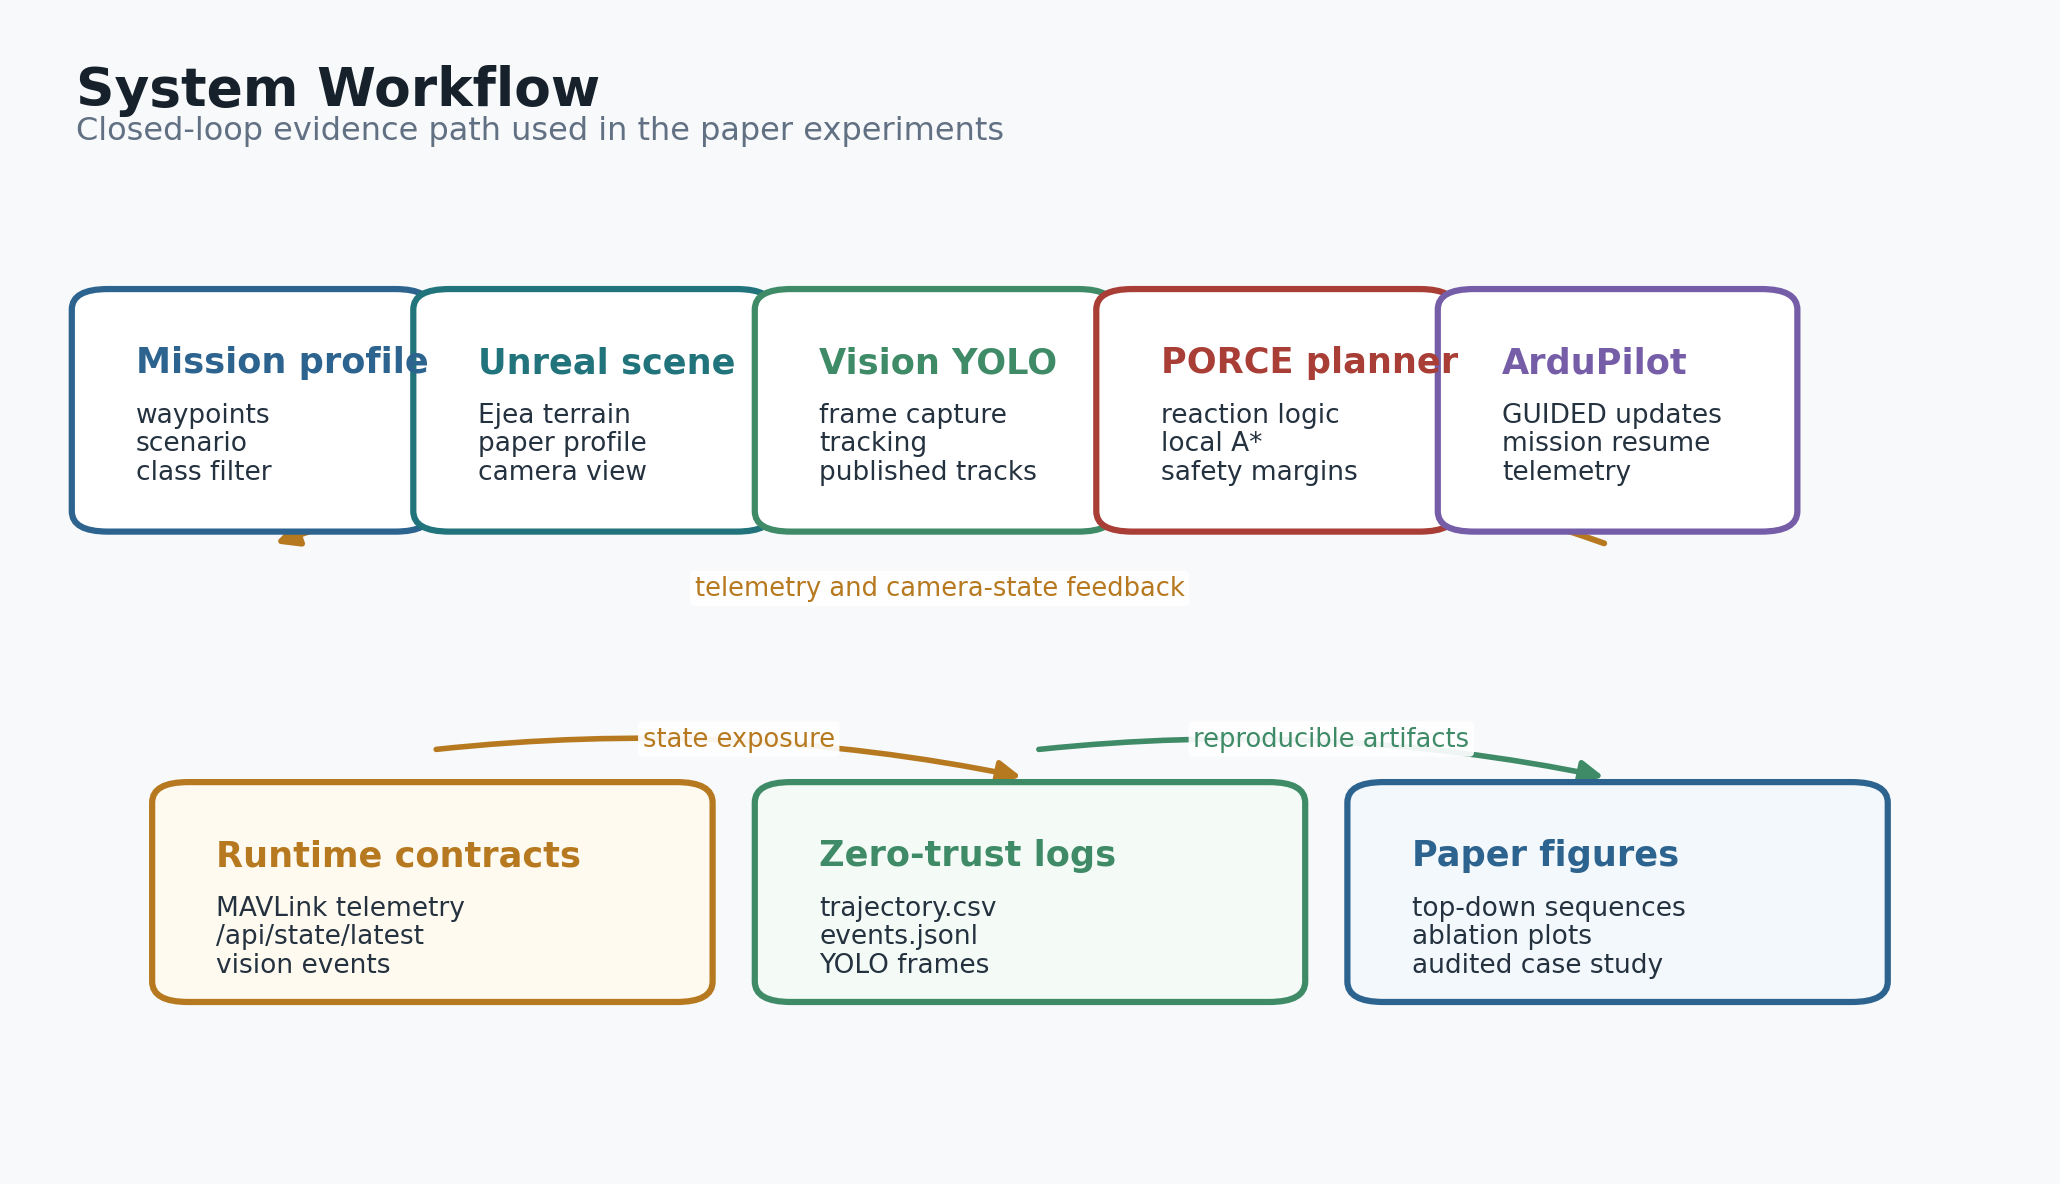
\includegraphics[width=\columnwidth]{Imagenes/System Workflow.png}
\caption{System Workflow}
\label{solution}
\end{figure}

However, as introduced in Section 2, the operational focus shifts during the execution phase. At this stage, residual risks can arise due to dynamic, uncertain, or locally perceived conditions that cannot be fully captured during the planning phase. In these circumstances, simplified assumptions and toy-problem formulation often emerge, together with a neglect of regulatory compliance considerations.The proposed local reactive navigation model enables realistic adaptation in real-time to the environment.


The controller-level logic that constitutes the scientific core of the proposed method is specified below. The method receives the active waypoint, fresh perception outputs, and current telemetry; canonicalizes human-adjacent detections into protected local regions; evaluates whether the nearest obstacle enters the dynamic reaction horizon; and either preserves nominal mission following or activates a bounded A* local bypass. Importantly, the same decision chain also defines the fallback behavior and the audit outputs, so the proposal is not just a path planner but a complete online conflict-resolution policy.


%XABI: \diagramplaceholder{Flujo metodológico del sistema: debería verse un diagrama de control con inicio en la actualización de telemetría, waypoint activo y tracks; después, la canonicalización de clases tipo person/bicycle/biker en regiones protegidas; a continuación, el cálculo del horizonte dinámico de reacción y una decisión binaria sobre si el obstáculo entra o no en ese horizonte. Si no entra, el sistema mantiene el seguimiento nominal; si entra, construye el subconjunto acotado del planificador, ejecuta el A* local y decide si la ruta local es válida. Si lo es, ejecuta subobjetivos y reengancha con el waypoint actual; si no lo es, activa la escalera de failsafe. En paralelo, el mismo diagrama debería mostrar qué eventos de auditoría se generan en cada rama.}

\subsection{Problem Formulation}

At each control iteration, PORCE knows the current vehicle state, the active mission waypoint, and the most recent obstacle list. The method is only concerned with the local subproblem: move from the current position to the current waypoint while avoiding the obstacle subset that lies inside a bounded planning neighborhood.

Let the vehicle position be \(p_t \in \mathbb{R}^2\), the current waypoint be \(w_t \in \mathbb{R}^2\), and the perceived obstacles at time \(t\) be \(\mathcal{O}_t = \{o_1,\dots,o_k\}\). Each obstacle is inflated by a hard safety radius \(R_s\), generating a non-flyable region
\begin{equation}
    \mathcal{Z}_{\mathrm{safe}}(o_i) = \{q \in \mathbb{R}^2 : \lVert q - p_{o_i} \rVert_2 \le R_s\}.
\end{equation}

The local free space is therefore
\begin{equation}
    \mathcal{F}_t = \mathbb{R}^2 \setminus \bigcup_{i=1}^{k} \mathcal{Z}_{\mathrm{safe}}(o_i).
\end{equation}

In the current implementation, \(R_s = \SI{12}{\meter}\), which turns safety into a hard geometric constraint instead of a soft penalty.

Earlier conceptual project notes also discussed more general continuous cost-shaping ideas, including barrier-style formulations, as possible future directions. They are not the subject of the present paper. The system analyzed here is the one actually implemented in the repository: a deterministic bounded grid planner with hard obstacle inflation and explicit failsafe escalation, not a Control Barrier Function controller or any other unimplemented continuous optimizer.

\subsection{Dynamic Triggering Logic}

The method is not permanently active. The controller computes a dynamic reaction horizon
\begin{equation}
    D_{\mathrm{react}}(t) =
    \mathrm{clip}\!\left(D_{\mathrm{base}} + k_v \lVert v_t \rVert_2,\,
    D_{\min},\, D_{\max}\right),
\end{equation}
where \(D_{\mathrm{base}}=\SI{45}{\meter}\), \(k_v=\SI{2.0}{\second}\), \(D_{\min}=\SI{45}{\meter}\), and \(D_{\max}=\SI{80}{\meter}\).

If the nearest perceived obstacle satisfies
\begin{equation}
    d_{\mathrm{nearest}}(t) \le D_{\mathrm{react}}(t),
\end{equation}
and the minimum replan interval has elapsed, PORCE requests a new local route from the replanning module. Otherwise, the vehicle continues nominal waypoint following.

\subsection{Bounded Local A* Planner}

The method uses a local occupancy grid centered on the vehicle. The validated configuration uses \(81 \times 81\) cells with \(\delta=\SI{6}{\meter}\) resolution, yielding a bounded search window that is compatible with online execution inside the control loop.

Each cell \(c_{ij}\) is labeled as free or occupied according to the inflated obstacle set:
\begin{equation}
    S(c_{ij}) =
    \begin{cases}
        1, & \text{if } c_{ij} \cap \left(\mathbb{R}^2 \setminus \mathcal{F}_t\right) \neq \varnothing,\\
        0, & \text{otherwise.}
    \end{cases}
\end{equation}

The local route is computed with A* \cite{hart1968formal} using Euclidean heuristic,
\begin{equation}
    f(n) = g(n) + h(n),
\end{equation}
where \(g(n)\) is the cost of the accumulated path and \(h(n)\) is the Euclidean distance to the local goal. Eight-connectivity is enabled, so the method can combine cardinal and diagonal moves while remaining on the grid.

The target of the method is always the \emph{current mission waypoint}. This detail is important: the local planner is not allowed to redefine the global mission, only to create a temporary bypass that lets the UAV return to the original corridor as soon as the conflict disappears.

\subsection{Nominal Navigation, Temporary Inhibition, and Route Reattachment}

One of the clearest implementation ideas is that the method should be understood as a \emph{temporary inhibition} of nominal navigation rather than as a new mission planner. 

Inside the control loop, the detection function is activated, so the system will continuously check the state of the obstacles with the detection function ($get\_detection$). The system responsible for providing the input to this function is an RGB camera on-boarded in the UAS. The methodology uses for detection of non regulatory compliant items or physical obstacles is based in the tracking proposed on \cite{alaez2023real}.

This detection function is the key element to select the path inside the control loop. If no conflict is detected, the system executes the nominal navigation flow, following the previously planned trajectory. The nominal navigation works as follows: 
\begin{itemize}
    \item If $current\_idx$ is less than the length of the proposed flight plan, the system continue with the planned flight path. At each iteration, it checks whether the distance to the current target waypoint is below a threshold tolerance ($WP\_TOLERANCE$); if so, the target is updated to the next waypoint for the subsequent iteration. 
    \item If not, it implies that the last waypoint of the Flight Plan is reached, so the mission terminates normally through the landing logic.
\end{itemize}

Conversely, When the nearest obstacle crosses the dynamic reaction horizon, this nominal flow is suspended, and an evasion path becomes the active short-horizon reference. During that interval, the aircraft no longer tries to cut through the original corridor; instead, it follows the local sub-goals returned by the bounded A* planner. As soon as that local path is exhausted, nominal waypoint following resumes automatically toward the same mission waypoint that was active before the conflict.

This behavior is operationally important for powerline inspection. The objective of the method is not merely to avoid collisions, but to resolve local conflicts in real time. Once safe conditions are restored, the system returns to the globally planned route as quickly as possible. In this way, operational safety is maintained without compromising the efficiency objective defined during the initial global planning stage, whether optimized data acquisition, mission progression, or any other mission-specific metric established a priori.

%PORCE: Vuelto a poner mezclado con las palabras que había inicialmente, pero se pueden mezclar ambas si se cree que falta algo por aportar. 
%This point is operationally important for inspection: the objective of the method is not just to avoid collision, but to resolve the local conflict while returning as quickly as possible to the globally planned route that was originally chosen to optimize data capture and mission progression.

\subsection{Failsafe Escalation}

If no valid local route is found, PORCE does not continue nominal flight blindly. Instead, the system integration includes an explicit escalation chain with hold, lateral replan, and terminal \texttt{LAND}/\texttt{RTL} actions. This failsafe design is part of the method even when it is not triggered in a particular experiment because it bounds the controller behavior under planner failure.

\subsection{Algorithmic Summary}

\begin{lstlisting}[language=Python, caption=Simplified control loop for the proposed method]
Flight_Plan = load_plan()
while Mission
    refresh_telemetry_and_obstacles()
    if telemetry_stale:
        continue

    if failsafe_action_active:
        execute_failsafe_action()
        continue

    wp = waypoints[current_wp_idx]
    reaction = clamp(base + groundspeed * gain,...
    min_r, max_r)
    nearest = nearest_obstacle()

    if nearest and nearest.dist < reaction and ...
    replan_allowed_now():
        route = astar_local(drone_pos, wp,... 
        planner_subset_obstacles())
        if valid(route):
            activate_evasion(route)
        else:
            apply_failsafe_escalation(nearest.dist)

    if evasion_active:
        follow_evasion_subpoints()
    else:
        follow_mission_waypoint(wp)
        if wp < length (Flight_Plan): 
            dist = get_WP_distance()
            if dist < WP_TOLERANCE_M
                current_wp_idx =+1
        else: 
            FlightMode = ['LAND']
            Mission = 0

\end{lstlisting}

\section{PORCE Integration in Simulation Workflow}

The proposed method is evaluated inside  the validated \texttt{SIMULATION} workflow in the repository \cite{Deep_Aero_Twin}. The runtime architecture is specified in the figure \ref{Simulation Environment Diagram}. The mission is read from a QGroundControl waypoint file, vehicle state is received from SITL through MAVLink, obstacles are produced by the vision module, and the PORCE system coordinates nominal waypoint following, replanning activation, and visualization outputs.

\begin{figure}[h!]
\centering
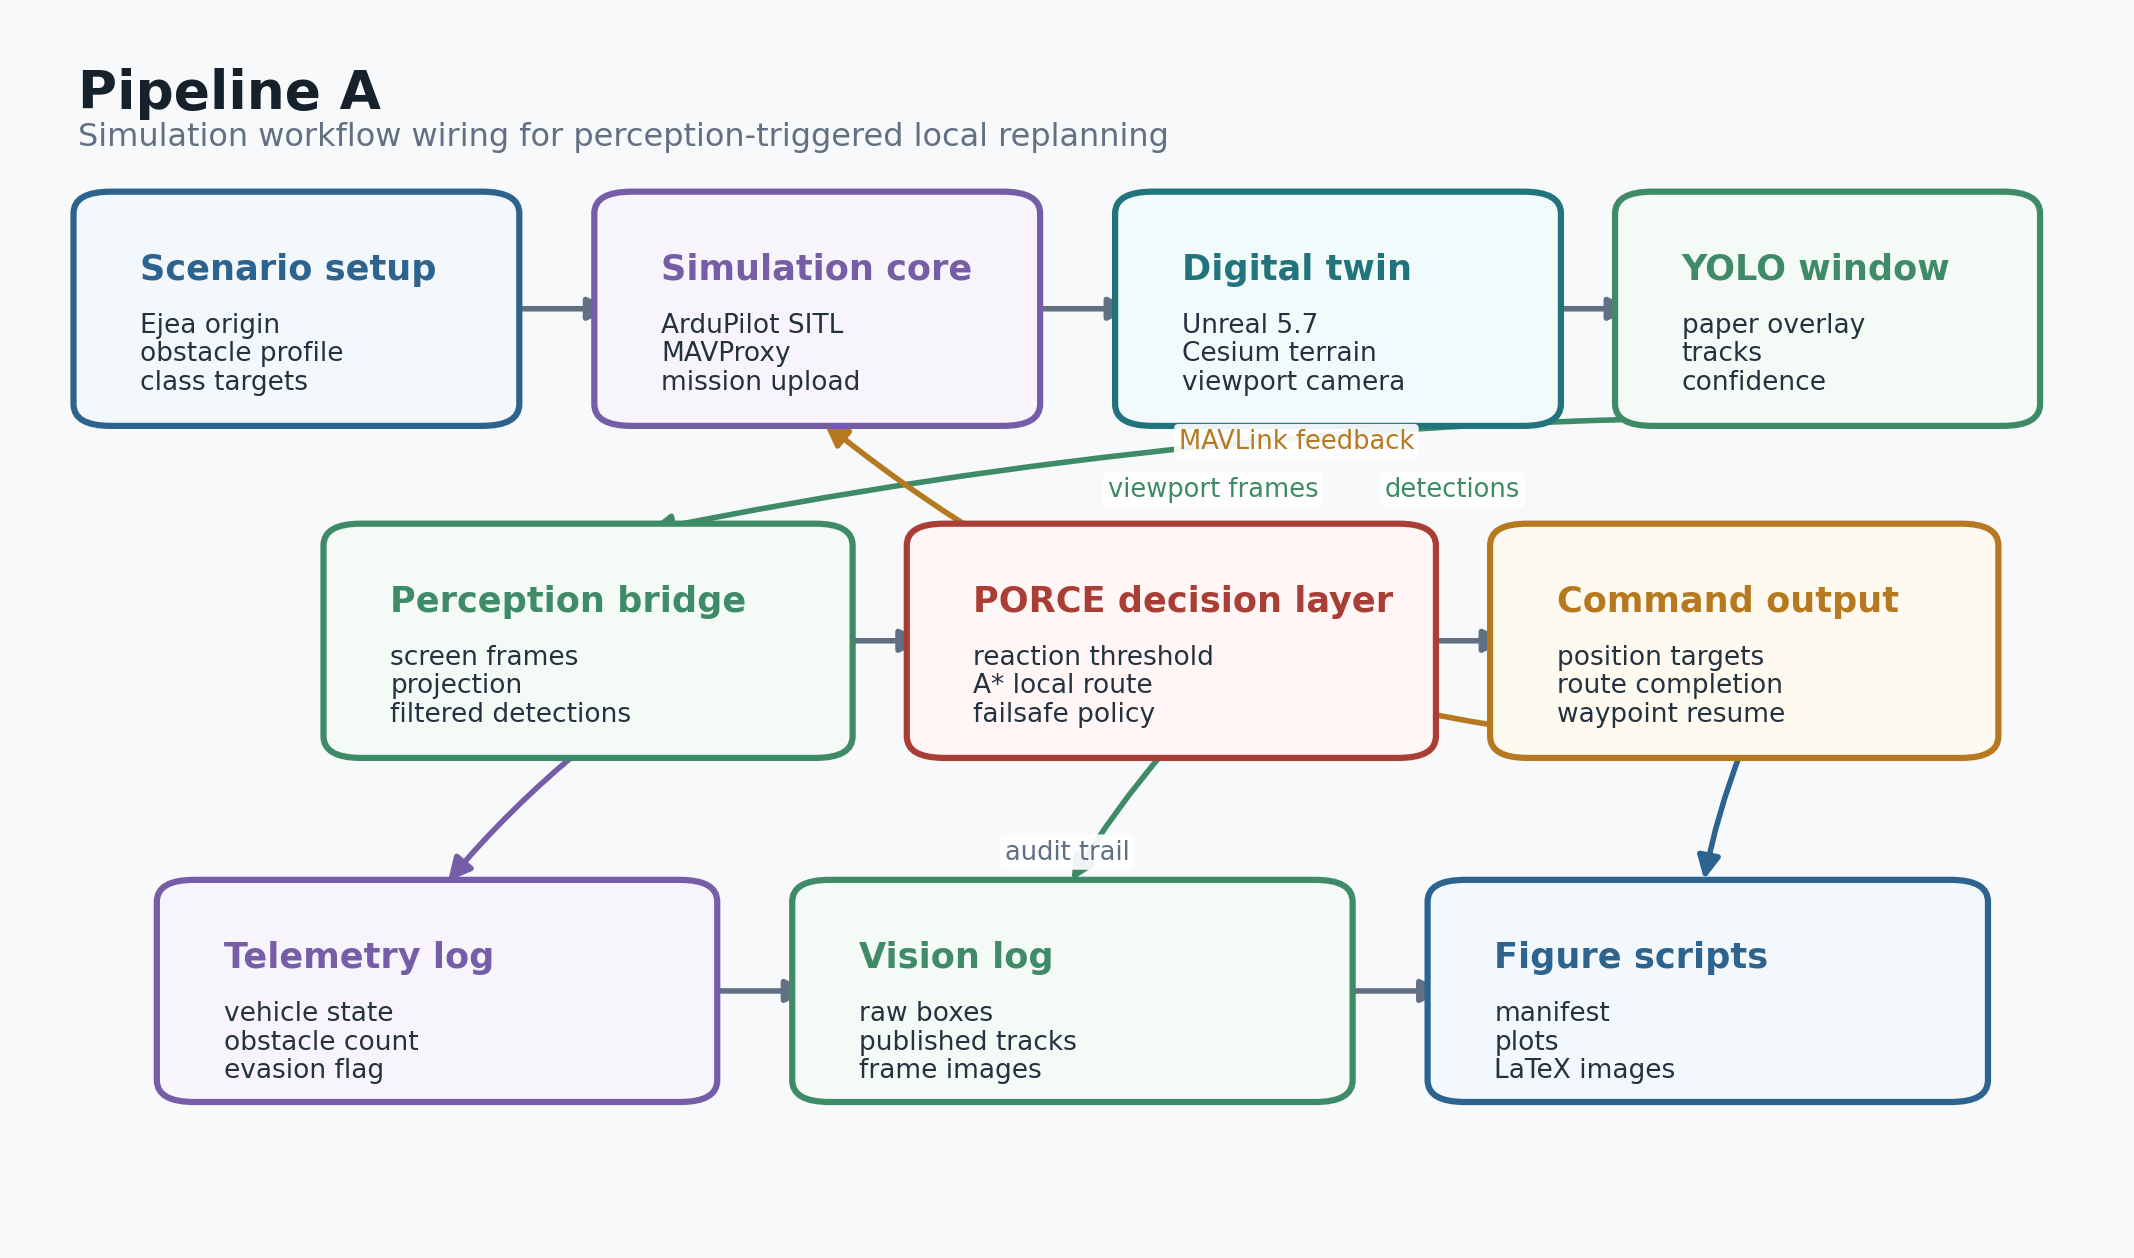
\includegraphics[width=\columnwidth]{Imagenes/Pipeline A.png}
\caption{Simulation Environment Diagram}
\label{Simulation Environment Diagram}
\end{figure}

%XABI: \diagramplaceholder{Arquitectura de Pipeline A: debería verse, de izquierda a derecha, la cadena completa de integración con el fichero de misión, la fuente visual Cesium/Unreal y la telemetría MAVLink entrando en el Brain; debajo, el sistema de visión devolviendo tracks geoposicionados; a la derecha, el planificador local de evasión entregando una ruta local y, más abajo, el autopiloto ejecutando setpoints; todavía más a la derecha, la API de estado compartido y los artefactos zero-trust como salida auditable. Las flechas deberían distinguir claramente flujo operativo en tiempo real frente a flujo de auditoría, sin cruces ni ambigüedades, para dejar inequívoco cómo se integra el sistema con Pipeline A.}

The Simulation Environment roles are the following:
\begin{itemize}
    \item \textbf{Mission input:} This is the file that contains the nominal inspection route.
    \item \textbf{SITL:}
    \item \textbf{MAVLINK Telemetry}:
    \item \textbf{Cesium / Unreal}: It is the visual Source of the environment. 
    \item \textbf{PORCE:} the PORCE system executes the control loop, manages waypoints, handles failsafe logic, and calls the replanning module whenever local replanning is necessary.
    \item \textbf{Perception:} This module runs a YOLO-based detector and projects detections in geographic coordinates using onboard state and the monocular geometry \cite{alaez2023real}. It is part of the PORCE control loop. 
    \item \textbf{Local Avoidance Planner:} This function implements the bounded A* local planner used to generate short-range evasion paths. It is part of the PORCE control loop. 
    \item \textbf{Visualization:} the visualization endpoint expose the evolution of the mission for analysis and debugging.
    \item \textbf{autopilot}: It runs inside SITL. Setpoint Execution. 
\end{itemize}

\subsection{Runtime Integration with Simulation Workflow}
The integration of the proposed method into Simulation Workflow is a closed-loop runtime contract rather than a loose module coupling. 
\newline
First, the mission is loaded from a QGroundControl waypoint file, and PORCE receives vehicle telemetry from SITL through MAVLink;
\newline 
Second, the perception subsystem queries the latest fused vehicle state and publishes detected obstacles to PORCE through \texttt{POST /api/obstacles}. PORCE then normalizes obstacle classes, enforces source filtering and token validation, maintains obstacle tracks with time-to-live logic, and rebuilds the active obstacle list used for decision making;
\newline
In the current implementation, human-adjacent detections are already given a dedicated operational treatment. The labels \texttt{person}, \texttt{bicycle}, and \texttt{biker} are canonicalized into the same moving obstacle family, while \texttt{tower} and \texttt{cow} are treated as static classes for tracking and association purposes. This is not yet a full legal ontology of uninvolved people, but it is the concrete mechanism by which civilian-like detections become protected local regions that the method must avoid rather than overfly;
\newline
Third, the method is only evaluated when the autonomous mission is active, fresh obstacle evidence exists, and the nearest obstacle crosses a speed-adaptive reaction horizon. Before invoking the planner, PORCE forms a subset of bounded obstacles for local replanning: in the validated configuration, only obstacles inside \SI{55}{\meter} and up to 16 tracks are passed to the planner. This keeps the replanning problem short-range and explicitly tied to the current mission waypoint instead of allowing corridor-wide route redefinition; 

\begin{table}[h!]
    \centering
    \small
    \begin{tabular}{@{}p{0.3\columnwidth} p{0.2\columnwidth} p{0.4\columnwidth}@{}}
        \toprule
        \textbf{Parameter} & \textbf{Value} & \textbf{Role} \\
        \midrule
        Mission file & 12 waypoints & Nominal inspection route with takeoff and landing phases \\
        Control-loop period & \SI{0.10}{\second} & PORCE update period \\
        Cruise speed & \SI{8}{\meter\per\second} & Nominal horizontal mission speed \\
        Grid cell size & \SI{6}{\meter} & Local A* discretization step \\
        Grid radius & 40 cells & Local search radius, i.e. an \(81 \times 81\) occupancy grid \\
        Obstacle safety radius & \SI{12}{\meter} & Hard inflation radius around each obstacle \\
        Base reaction distance & \SI{45}{\meter} & Minimum horizon for replanning activation \\
        Reaction gain & \SI{2.0}{\second} & Speed-dependent enlargement of reaction horizon \\
        Reaction range & \SIrange{45}{80}{\meter} & Clamped reaction distance interval \\
        Route-point tolerance & \SI{3}{\meter} & Distance to accept a local replanning sub-goal as reached \\
        Failsafe threshold & \SI{22}{\meter} & Distance used for hold/lateral replan escalation \\
        Failsafe hold & \SI{2.5}{\second} & Temporary hold action when replanning fails \\
        \bottomrule
    \end{tabular}
    \caption{Main configuration values of the validation environment and the proposed method used throughout the paper.}
    \label{tab:config}
\end{table}

Fourth, PORCE calls a specific function, where the start is the current telemetry position and the goal is the current mission waypoint. The planner inflates each obstacle by the configured safety radius, discretizes the neighborhood into a local \(81 \times 81\) occupancy grid with \SI{6}{\meter} cells, runs bounded A*, and converts the resulting grid path back into geographic sub-points. If a valid route is found, PORCE stores it as the active evasion path; if not, the integration layer escalates through hold, lateral replan, and terminal failsafe actions;
\newline

Finally, the method outputs are consumed by the rest of the Simulated Environment through two channels. On the control side, PORCE sends each local replanning sub-point to the autopilot as MAVLink position-target commands until the evasion route is completed, at which point nominal waypoint following resumes automatically. On the observability side, the same state is exposed through the UI endpoint together with evasion metadata, planner parameters, tracked obstacles, and audit counters, so visualization tools, Unreal consumers, and zero-trust logs all observe the same decision chain. This shared contract is what makes the method not just a planner in isolation, but a reproducible system integrated into a full autonomous inspection pipeline.


Table~\ref{tab:config} summarizes the main runtime parameters used to evaluate the method inside the Simulation Workflow. These values come from the validated simulation defaults already present in the repository.

\section{Results}

In this section, the results of the experiments performed with the environment present in the $Deep\_Aero\_Twin$ repository using the proposed method are represented. 

In a first step, the Mission is downloaded into the simulated UAS. The mission comes from a preplanned waypoints file that contains a takeoff waypoint, a sequence of predefined inspection waypoints and a landing command. For the experiment, the UAS clims from \SI{500}{\meter} MSL to approximately \SI{523}{\meter} MSL, follows the inspection corridor, and lands automatically once the final waypoint is reached. This initial planned behaviour is represented in Figure \ref{instante inicial}, where it is appreciable that at in the initial stages, the UAS is navigating without any perturbation, following the predefined waypoints path. 

%AQUÍ LA FIGURA 1 con los 6 casos del ejemplo estático. 
%1A, 1B y 1C en la primera fila y 1D, 1E y 1F en la segunda fila. La imagen 1A y 1D son representaciones gráficas y la imagen 1B-1E y 1C-1F son parejas de imágenes en las que arriba sale la representación del caso en unreal y abajo la representación del caso en una gráfica. 

%Figura 1A: Ejemplo inicial en el que el UAS está siguiendo la "Nominal Navigation" con los waypoints predefinidos y sin ningún cambio. 

%Figura 1D Estado completo de la ruta en resumen en la que se vean todas las evasiones que ha ido haciendo y el resumen de la ruta (sobre la que debería haber sido originalmente y la que ha seguido en realidad. 

%Figura 1B: Se encuentra en el estado de detección pero todavía no está a la distancia de seguridad como para ejecutar la acción (representación unreal).

%Figura 1E: Se encuentra en el estado de detección pero todavía no está a la distancia de seguridad como para ejecutar la acción (representación grafica).

%Figura 1C: Se encuentra ya en el estado de evasión en el que el grid ha salido y se está ejecutando la maniobra evasiva. Representación unreal (con un zom a lo que está pasando en el esquive). 

%Figura 1F: Se encuentra ya en el estado de evasión en el que el grid ha salido y se está ejecutando la maniobra evasiva. Representación gráfica  (con un zom a lo que está pasando en el esquive). 






% Falta la figura 1F que la dejamos por si hay alguno de los casos que creas conveniente resaltar en 

\begin{figure}[h!]
\centering
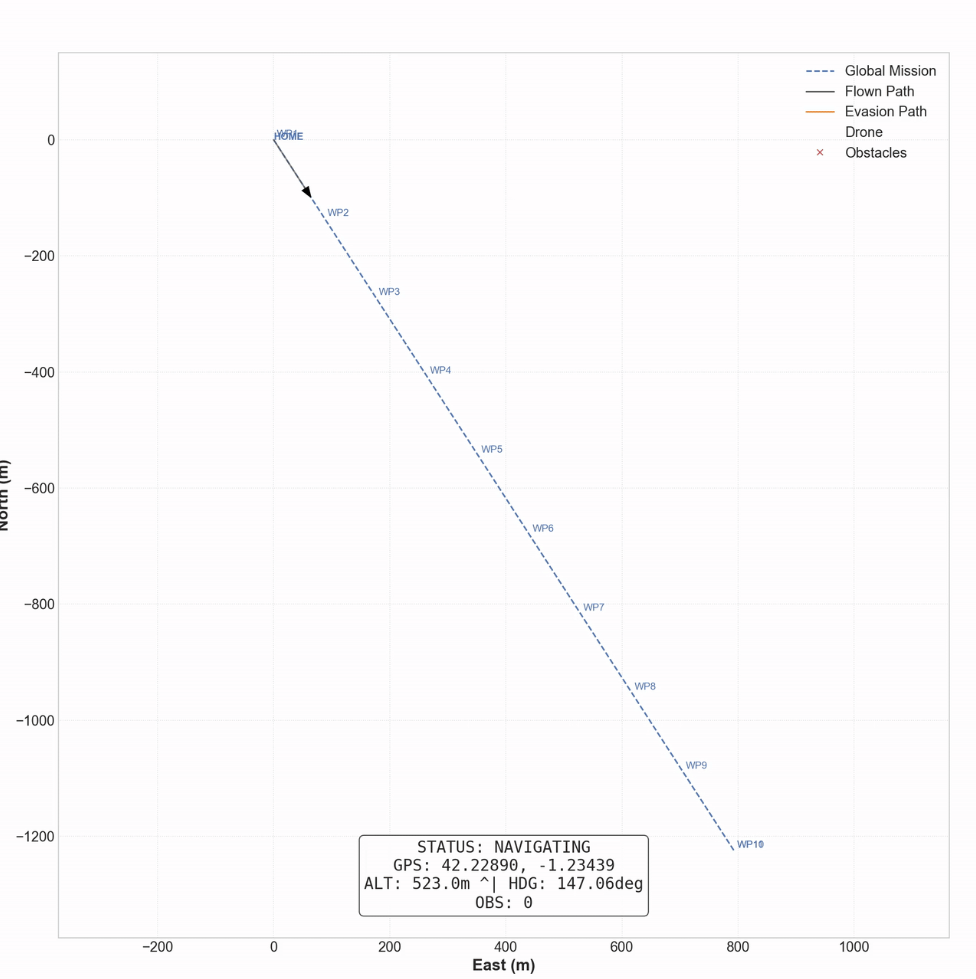
\includegraphics[width=\columnwidth]{Imagenes/Instante_inicial_del_recorrido.png}
\caption{Initial Stages. Nominal Navigation}
\label{instante inicial}
\end{figure}
 

As explained before, while the UAS is in the air and, therefore, the proposed solution is running inside the embedded computer, the system is continuously analyzing the environment to detect if there is any obstacle or non regulatory compliant item that needs to be avoided. In Figure \ref{deteccion pero no dentro de margen}, it is represented the instant where the camera has already detected an obstacle (i.e. the obstacle is inside the Reaction Range), but the distance between the UAS and the obstacle is more than the Base Reaction Distance. Therefore, the system is not calculating yet an alternative evasion path, as the obstacle is only a potential hazard yet. 

\begin{figure}[h!]
\centering
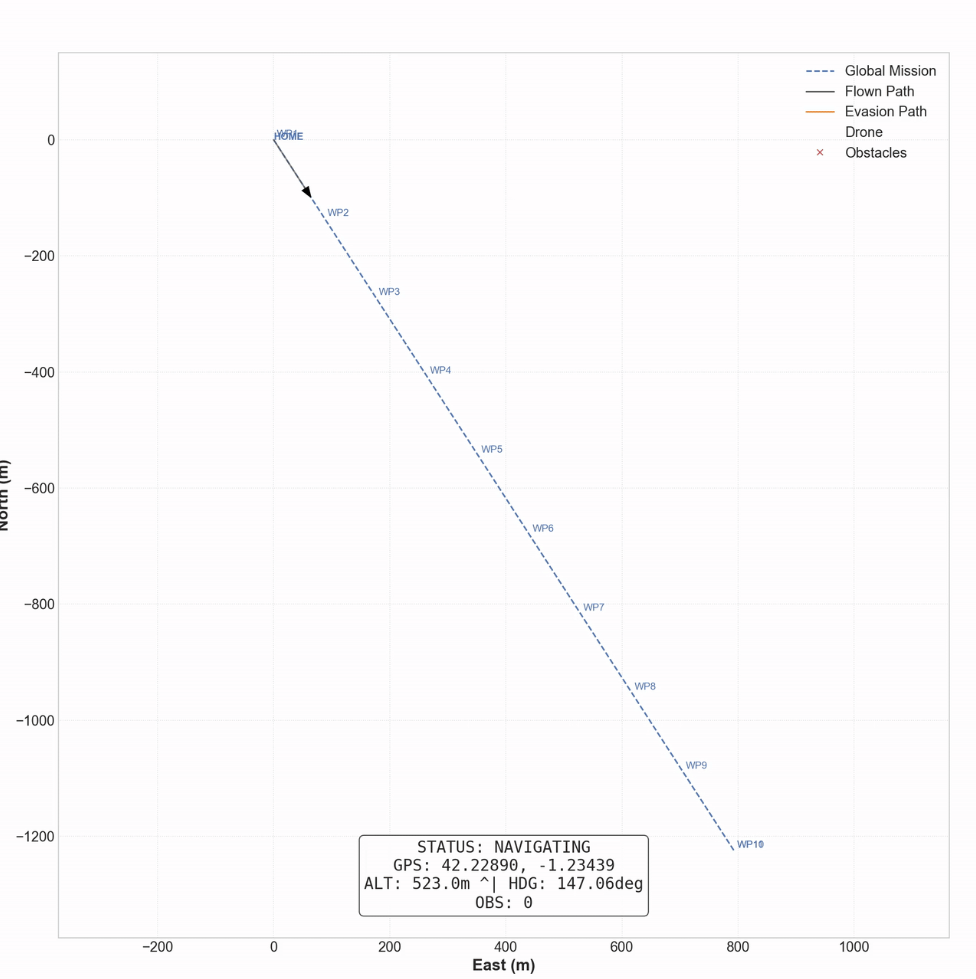
\includegraphics[width=\columnwidth]{Imagenes/Instante_inicial_del_recorrido.png}
\caption{Detection Stage. No safety action}
\label{deteccion pero no dentro de margen}
\end{figure}


In contrast to the previous paragraph and figure, where the obstacle had already been detected but remained outside the safety radius, the following figure represents a later stage of the encounter. At this instant, the obstacle has entered the reaction distance, triggering the trajectory replanning process. As a result, the system begins to compute an avoidance route intended to prevent a potential conflict and preserve the required separation margins.


\begin{figure}[h!]
\centering
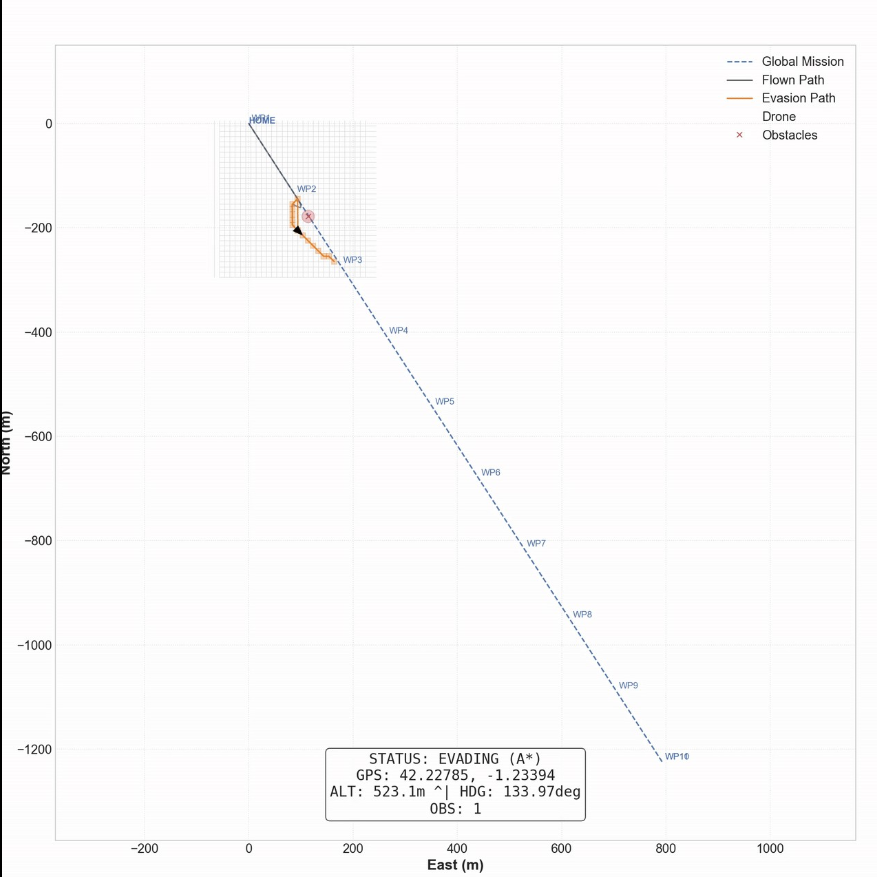
\includegraphics[width=\columnwidth]{Imagenes/instante_durante_evasion.png}
\caption{Evasion Stage. Safety action}
\label{deteccion dentro del margen}
\end{figure}

The route proposed by the UAS is highlighted in orange, allowing the guidance response to be clearly distinguished from the original trajectory. This visualization therefore illustrates the transition from a passive monitoring state, in which the obstacle is detected but no corrective action is required, to an active guidance state, in which the system evaluates the conflict and generates a feasible alternative path.

%PORCE: Faltaría en algún punto una descripción de la visualización del grid. La teoría que se ha explicado con anterioridad se ve reflejado en la imagen, con lo cual es representativo de lo que realiza la solución de evasión PORCE. 

\begin{figure}[h!]
\centering
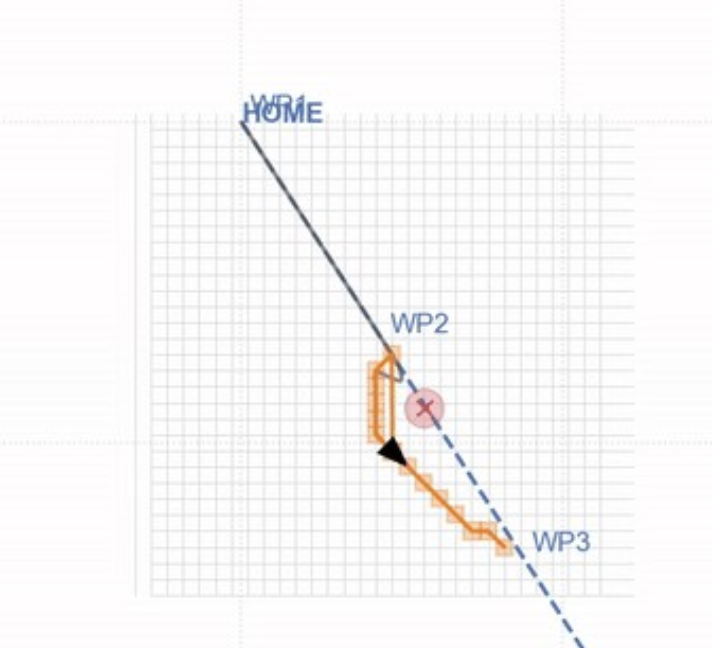
\includegraphics[width=\columnwidth]{Imagenes/instante_durante_evasion_zoom.png}
\caption{Evasion Stage. Safety action}
\label{deteccion dentro del margen}
\end{figure}

\newpage

Figure \ref{vuelta al path y nueva deteccion} shows the complete resolution of the conflict, once the UAS has successfully rejoined its original path and can continue with the data acquisition mission. At this stage, the avoidance maneuver has been completed and the vehicle has returned to nominal operation, resuming the planned inspection or monitoring task. This moment represents the final phase of the guidance response, where the temporary deviation introduced to maintain safe separation is no longer required and the mission can proceed under normal conditions.

At this point, the incident is also recorded and reported by the system for subsequent analysis. Although this may result in partial data loss or gaps in the information collected from the asset during the maneuver, such limitations are considered acceptable within the operational framework. In safety-critical applications, preserving the integrity of the UAS and maintaining a safe distance from obstacles must take precedence over uninterrupted data collection. Therefore, the figure not only illustrates the successful completion of the conflict-resolution process, but also highlights the underlying operational principle that mission continuity is always subordinated to safety requirements.

\begin{figure}[h!]
\centering
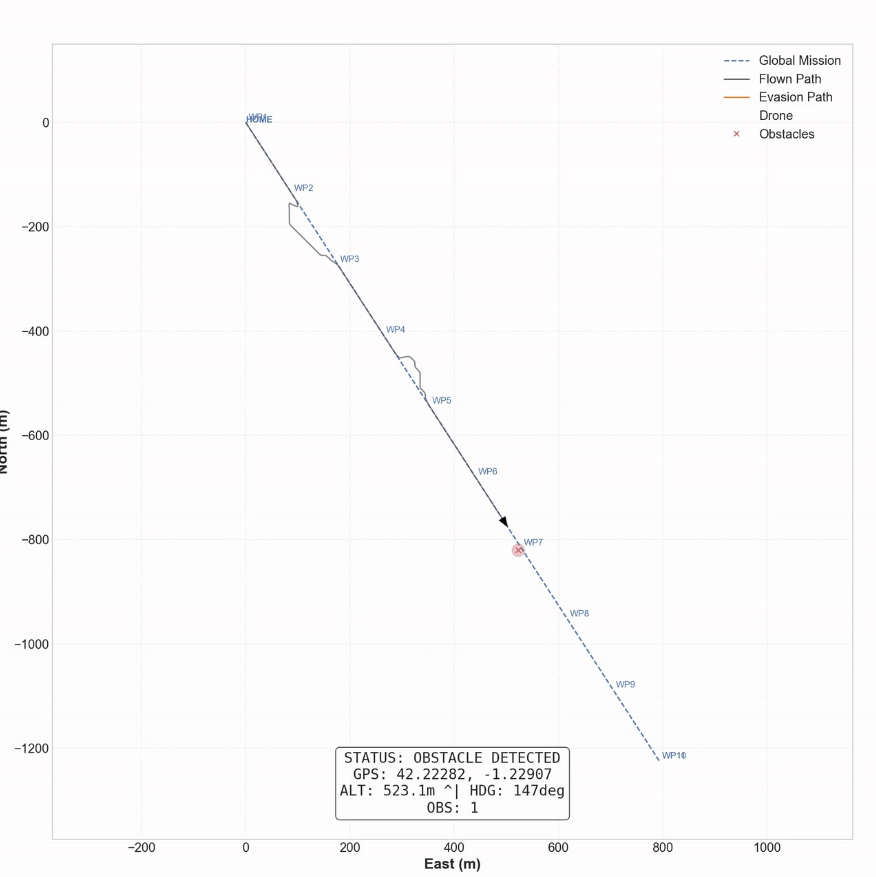
\includegraphics[width=\columnwidth]{Imagenes/transcurso_de_mision_(nuevo_obs_detectado).png}
\caption{Middle Stages. Re-joining and new detections }
\label{vuelta al path y nueva deteccion}
\end{figure}

Moreover, Figure \ref{vuelta al path y nueva deteccion} also shows that the process does not remain as an isolated event. A new detection can be observed after the UAS has returned to its nominal trajectory, demonstrating that the system is not limited to a single conflict-resolution cycle. Instead, it is capable of repeatedly transitioning between normal path-following, obstacle detection, trajectory replanning, and recovery to the original route as many times as required by the operational scenario. This behavior confirms the robustness and repeatability of the guidance strategy, showing that the UAS can respond consistently to successive conflicts without any inherent limitation in its ability to resume the mission and reinitiate the avoidance process whenever necessary.


Finally, in Figure \ref{fase final. Completado} the final stage of the process is shown once the UAS has reached the final position and is performing the landing phase. In this figure, it can be appreciated the representativeness of the solution, as the route is not fully straight as preplanned, due to the different detections and re-routing stages that the UAS has experimented during its simulated mission. %PORCE: Falta que la figura ponga landing stage al final del todo, en vez de seguir navegando. 


\begin{figure}[h!]
\centering
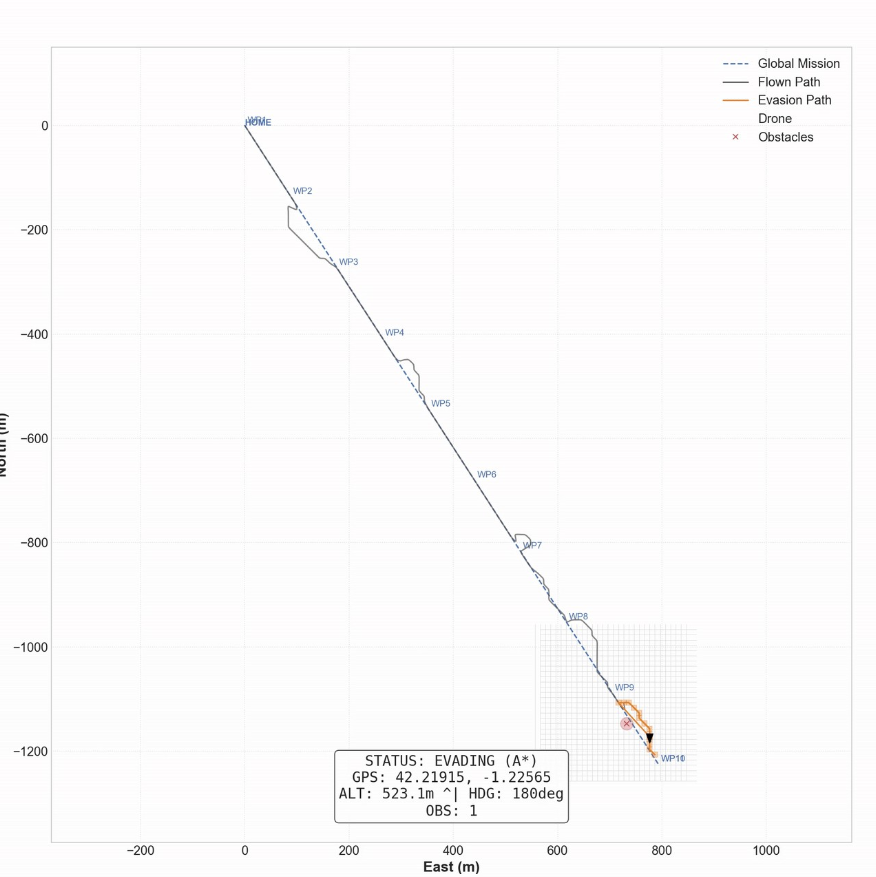
\includegraphics[width=\columnwidth]{Imagenes/ruta_completada_ultimo_obs.png}
\caption{Final Stage. Landing }
\label{fase final. Completado}
\end{figure}

%PORCE: Para mi dentro de esta parte de metodología experimental sobra la parte de auditoría. Habría que adaptarlo a la propuesta de sacar las diferentes capturas del Gif para explicar como funciona la metodología. Y ya ver si eso si meter algo de lo que ha propuesto Xabi de la parte del E2E. Pero eso quizás a él le da para otro artículo y no es necesario meterlo por aquí.

%%PORCE: PROPUESTA DE XABI

\section{Experimental Methodology}

\subsection{Evidence Sources}

The paper uses two complementary evidence sources already present in the repository.

\begin{itemize}

    \item \textbf{Controlled E2E ablations:} four mission logs from \texttt{pipeline/logs/e2e/} comparing the replanning module enabled or disabled, with and without detections.
    \item \textbf{Audited case study:} one clean zero-trust run (\texttt{20260220\_092802}) with trajectory logs, PORCE events, and per-frame vision audit payloads.
\end{itemize}

The E2E ablation isolates the behavioral effect of enabling the method under detections. The zero-trust run provides richer observability: trigger distance, generated route length, evasion duration, obstacle tracks, and the complete time evolution of the maneuver. However, the event \texttt{evasion\_route\_generated} stores \texttt{planner\_obs\_count} but not the exact obstacle identities passed to the planner. Therefore, all post-hoc clearance analysis in this paper is computed against the nearest published trigger-side tracks in the last pre-trigger vision frame, which is the closest auditable proxy available in the repository.

\subsection{Mission and Metrics}

The mission comes from \texttt{pipeline/ejea\_default.waypoints}. It contains a takeoff waypoint, a sequence of inspection waypoints, and a landing command. For all experiments, the UAV climbs from \SI{500}{\meter} MSL to approximately \SI{523}{\meter} MSL, follows the inspection corridor, and lands autonomously once the final waypoint is reached.

The following metrics are extracted from logs:
\begin{itemize}
    \item mission duration, measured from the first to the last status sample in the E2E logs;
    \item path length, computed by summing point-to-point geodesic distances along the logged trajectory;
    \item trigger distance, route-point count, and evasion duration from \texttt{events.jsonl};
    \item minimum geometric separation between the executed evasion trajectory and the closest auditable proxy of the planner subset at trigger time;
    \item detour cost, computed as the difference between evasion path length and the straight-line segment joining the first and last evasion points.
\end{itemize}

The visual materials discussed in the paper were generated directly from repository logs by a dedicated script placed inside the \texttt{paper/} folder. In the present draft, the still-pending diagrams are replaced by short placeholder paragraphs in Spanish that specify the exact visual evidence expected in the final version, so the results section remains reproducible from project artifacts even before the final artwork is rebuilt.

\section{Experimental Validation of the Proposed Method}

\subsection{Controlled E2E Ablation}

The early section of the E2E trajectories is specified below through a short placeholder paragraph in Spanish while the final plot is being rebuilt. The two scenarios without detections are practically identical regardless of whether the replanning module is enabled, which confirms that the planner remains dormant when no conflict enters the system. The \texttt{replanner off + detections} scenario also follows the nominal corridor, while \texttt{replanner on + detections} introduces a visible local detour before rejoining the original path.

%XABI: \diagramplaceholder{Ablación E2E de trayectorias: debería verse una superposición de las cuatro trayectorias del tramo inicial de misión, con colores claramente diferenciados para \texttt{replanner on/off} y \texttt{detections on/off}. El mensaje visual que debe quedar claro es que los dos casos sin detecciones casi se solapan por completo, que el caso con detecciones pero el replanning desactivado sigue el corredor nominal, y que solo el caso con detecciones y el replanning activado introduce un desvío local corto antes de reincorporarse a la ruta original.}

Table~\ref{tab:e2e} quantifies this result. The mission always completes, and the overhead introduced by the avoidance behavior is small: relative to \texttt{replanner off + detections}, enabling the method under detections adds only \SI{4.6}{\meter} to the path and \SI{2}{\second} to the total mission.

\begin{table}[t]
    \centering
    \small
    \begin{tabular}{@{}p{0.43\columnwidth} S[table-format=3.0] S[table-format=4.1] c@{}}
        \toprule
        \textbf{Scenario} & {\textbf{Time (s)}} & {\textbf{Path (m)}} & \textbf{Done} \\
        \midrule
        replanner on + detections & 206 & 1460.1 & Yes \\
        replanner off + detections & 204 & 1455.5 & Yes \\
        replanner on + no detections & 204 & 1455.6 & Yes \\
        replanner off + no detections & 204 & 1455.6 & Yes \\
        \bottomrule
    \end{tabular}
    \caption{Controlled E2E ablation metrics extracted from \texttt{pipeline/logs/e2e}.}
    \label{tab:e2e}
\end{table}

This ablation does not claim broad statistical superiority; instead, it verifies a narrower but operationally important property of the proposed method: the system is behaviorally specific. It perturbs the mission only when both conditions hold simultaneously, namely obstacle evidence is present and the replanning module is enabled.

\subsection{Audited Collision-Evasion Maneuver}

The selected zero-trust maneuver comes from run \texttt{20260220\_092802} and is intentionally stricter than the earlier tower/cattle-like cases because the trigger-side detections are \texttt{biker} tracks, i.e. the human-adjacent obstacle family that most directly supports the no-overflight claim of the proposed method. The perception-to-planner chain is specified below through a short placeholder paragraph in Spanish while the final montage is being rebuilt: from the last pre-trigger vision frame (frame 5053 at \(t=-\SI{0.095}{\second}\)), 300 raw detector boxes are reduced to 233 projected detections, then to four published \texttt{biker} tracks, of which the three nearest are used as the auditable proxy of the planner subset. This is the strongest zero-trust reconstruction possible from repository artifacts because the route event serializes the planner count but not the obstacle identities.

%XABI: \diagramplaceholder{Montaje de percepción a planificador: debería verse, en la parte superior, una secuencia de reducción con cuatro etapas claramente numeradas: 300 cajas brutas, 233 detecciones proyectadas, 4 tracks \texttt{biker} publicados y 3 tracks finales usados como proxy del subconjunto del planificador. En la parte inferior deberían aparecer tres vistas coordinadas del mismo instante: espacio de píxel, espacio métrico local y espacio de rejilla del planificador. El objetivo visual no es estético sino probatorio: demostrar cómo la evidencia bruta termina convirtiéndose en la entrada auditable que realmente condiciona la activación del método.}

The geometric effect of the method in a local ENU frame centered on the trigger-side telemetry state is specified below through a short placeholder paragraph in Spanish while the final trajectory figure is being rebuilt. The background lattice matches the real \SI{6}{\meter} planner discretization, while the shaded occupied cells correspond to the auditable proxy obtained by inflating the three nearest published trigger-side \texttt{biker} tracks with the configured \SI{12}{\meter} safety radius. Two of those tracks, at 42.0 and \SI{42.1}{\meter}, quantize to the same seed cell, so the merged occupied block is a genuine property of the planner discretization rather than a drawing artifact. The vehicle then departs from the nominal mission corridor, executes a bounded bypass, and rejoins the original path before continuing toward WP9.

%XABI: \diagramplaceholder{Trayectoria auditada del caso: debería verse un plano local ENU con la rejilla real de \SI{6}{\meter} del planificador, el punto de disparo de la maniobra, el waypoint objetivo WP9, el segmento nominal de misión y la trayectoria ejecutada por el dron durante la evasión. También deberían verse las celdas ocupadas derivadas de inflar con \SI{12}{\meter} los tres tracks \texttt{biker} más cercanos, así como la ruta discreta de 15 puntos que recorre el planificador para rodear esa ocupación y volver a engancharse con el corredor nominal. El mensaje visual clave es que el desvío está cuantizado en la rejilla real y no en una rejilla arbitraria dibujada a posteriori.}

The geometric view is complemented below by a short placeholder paragraph in Spanish that specifies the expected time-series visualization while the final plot is being rebuilt. The reaction horizon remains comfortably above the clearance signal throughout the event, while the reconstructed geometric distance to the trigger-side proxy tracks never crosses the hard \SI{12}{\meter} safety radius. It does, however, fall below the \SI{22}{\meter} failsafe threshold during part of the maneuver, which is consistent with the role of that threshold as an escalation parameter for replanning failure rather than a guaranteed obstacle-clearance margin.

%\XABI: diagramplaceholder{Serie temporal de la maniobra: debería verse un eje temporal con, como mínimo, cuatro curvas o referencias claramente distinguibles: el horizonte dinámico de reacción, la distancia geométrica mínima a los tracks proxy, el radio duro de seguridad de \SI{12}{\meter} y el umbral de failsafe de \SI{22}{\meter}. Idealmente se marcarían también el instante de activación del método, la fase de evasión activa y el momento de reincorporación a la misión. La lectura visual que debe sostener la figura es que el sistema trabaja dentro de un margen estrecho pero auditable: nunca viola el radio duro de seguridad aunque sí entra en la zona que justificaría una escalada si el replanning fracasara.}

Table~\ref{tab:case} summarizes the main metrics derived from the audited run. The method is triggered at \SI{19.47}{\meter}, well inside the observed reaction horizon. It computes a 15-point local route and completes the maneuver in \SI{33.95}{\second}. The evasion path length is \SI{110.49}{\meter}; the equivalent straight-line segment between the first and last evasion points is \SI{43.60}{\meter}, so the local safety maneuver introduces a detour of \SI{66.90}{\meter}. Most importantly, the minimum geometric separation to the three trigger-side \texttt{biker} proxy tracks is \SI{13.48}{\meter}, which leaves only \SI{1.48}{\meter} of margin above the configured safety radius. That narrow but auditable clearance is scientifically stronger than an easy case because it shows the method operating close to the configured protection limit without crossing it.

\begin{table}[t]
    \centering
    \small
    \begin{tabular}{@{}p{0.68\columnwidth} S[table-format=3.2]@{}}
        \toprule
        \textbf{Metric} & {\textbf{Value}} \\
        \midrule
        Trigger distance (m) & 19.47 \\
        Published \texttt{biker} tracks in pre-trigger frame & 4 \\
        Trigger-side proxy obstacles & 3 \\
        Local route points & 15 \\
        Evasion duration (s) & 33.95 \\
        Maximum reaction distance during maneuver (m) & 61.11 \\
        Minimum geometric distance to planner-proxy tracks (m) & 13.48 \\
        Clearance above safety radius (m) & 1.48 \\
        Evasion path length (m) & 110.49 \\
        Straight-line equivalent (m) & 43.60 \\
        Local detour over straight segment (m) & 66.90 \\
        \bottomrule
    \end{tabular}
    \caption{Main audited metrics for run \texttt{20260220\_092802}.}
    \label{tab:case}
\end{table}

Together, the ablation and the audited case study support two claims. First, the method is selective: it does not inject unnecessary motion when obstacle evidence is absent. Second, when it does intervene, it produces a bounded and interpretable geometric deviation rather than a wholesale mission rewrite. For a power-line inspection workflow, this combination of selectivity, recoverability, and auditability is at least as important as raw avoidance capability.

% PORCE: Esta sección de limitaciones y Trabajo futuro me parece que está correcta y recoge la idea del artículo. Darle una vuelta a los puntos para darle un toque más humano. 

\section{Limitations and Future Work}

The current paper is intentionally aligned with the evidence already available for the proposed method in the repository, and this imposes clear limits on what can be claimed.
\begin{itemize}[leftmargin=1.3em]
    \item The experiments are simulation-based. The method is validated in Pipeline A under \texttt{SIMULATION}, but the real-world workflow still requires dedicated flight campaigns.
    \item The quantitative section is reproducible but not yet statistical. The paper reports representative runs and controlled ablations, not a large benchmark suite across many random seeds or scenarios.
    \item The regulatory novelty is operational rather than juridically complete. The method currently approximates uninvolved civilians through human-adjacent moving obstacle classes and conservative geometric avoidance; it is not yet a full SORA-compliant optimizer with class-dependent legal mitigations.
    \item The exact planner obstacle identities are not yet serialized in \texttt{evasion\_route\_generated}. Consequently, the paper reconstructs post-hoc clearance against the nearest published trigger-side tracks, which is the best auditable proxy but still weaker than logging the exact obstacle IDs passed to the replanning module.
    \item Perception uncertainty is only partially represented through the detector and geopositioning chain. Future experiments should characterize measurement error, missed detections, and class-dependent inflation policies more rigorously.
\end{itemize}

The next development steps are therefore clear: integrate broader scenario sets, add runtime measurements on representative onboard hardware, encode class-dependent safety envelopes for humans and other critical entities, and transfer the same methodology to the \texttt{REAL\_TWIN} and real-flight workflows.

%PORCE: Dar una vuelta a la conclusión pero como idea está bien fundamentada. De nuevo revisar para darle un toque más humano. Y quitar las referencias al E2E y la auditoría. 

\section{Conclusion}

This paper turns PORCE into the explicit scientific center of the manuscript and bases its characterization on evidences from the repository \cite{Deep_Aero_Twin}. The method is a bounded A* local replanning method that reacts only when necessary, preserves conservative geometric margins, and returns to the global mission once the conflict is resolved. Its specific contribution is not to claim that obstacle avoidance itself is novel, but to show how a local replanner can be shaped by the European ground-risk logic that discourages exposing uninvolved people and protected ground areas to unnecessary overflight. Pipeline A, in turn, provides the integrated simulation environment in which this behavior can be observed, audited, and measured.

The controlled E2E ablation shows that the overhead of enabling the method under detections is small, while the audited case study demonstrates that the method can generate and execute a complete local bypass with a narrow but explicit safety margin above the configured protection radius. Therefore, the strongest publishable claim is also the most precise one: to the best of our knowledge after reviewing recent 2024--2026 literature, the method represents the current state of the art for the narrowly defined problem of EASA-motivated, uninvolved-people-aware, deterministic controller-level local replanning inside an autonomous power-line inspection pipeline. Stated this way, the claim is ambitious but not misleading, because it does not assert superiority over all avoidance planners or all risk-aware route optimizers; it asserts leadership in the specific intersection that the system actually implements and documents.


\section*{Acknowledgment}

\bibliographystyle{ieeetr}
\bibliography{bibliografia/referencias_revision_porce}

ov\end{document}
